\subsection{Velocity Calibration}

First the MCS has to be calibrated, in order to transfer channel numbers to velocities.\\
With the given formula:
$$v[i] = \frac{\lambda}{2} \frac{N[i]}{N[2] \cdot 10} \text{mm} / \text{s}$$
and the additional information, that the range is traversed from maximum positive to maximum negative velocity and back, the relation illustrated in fig(\ref{fig:vcal}) is found.

\begin{figure}
\label{fig:vcal}
\centering
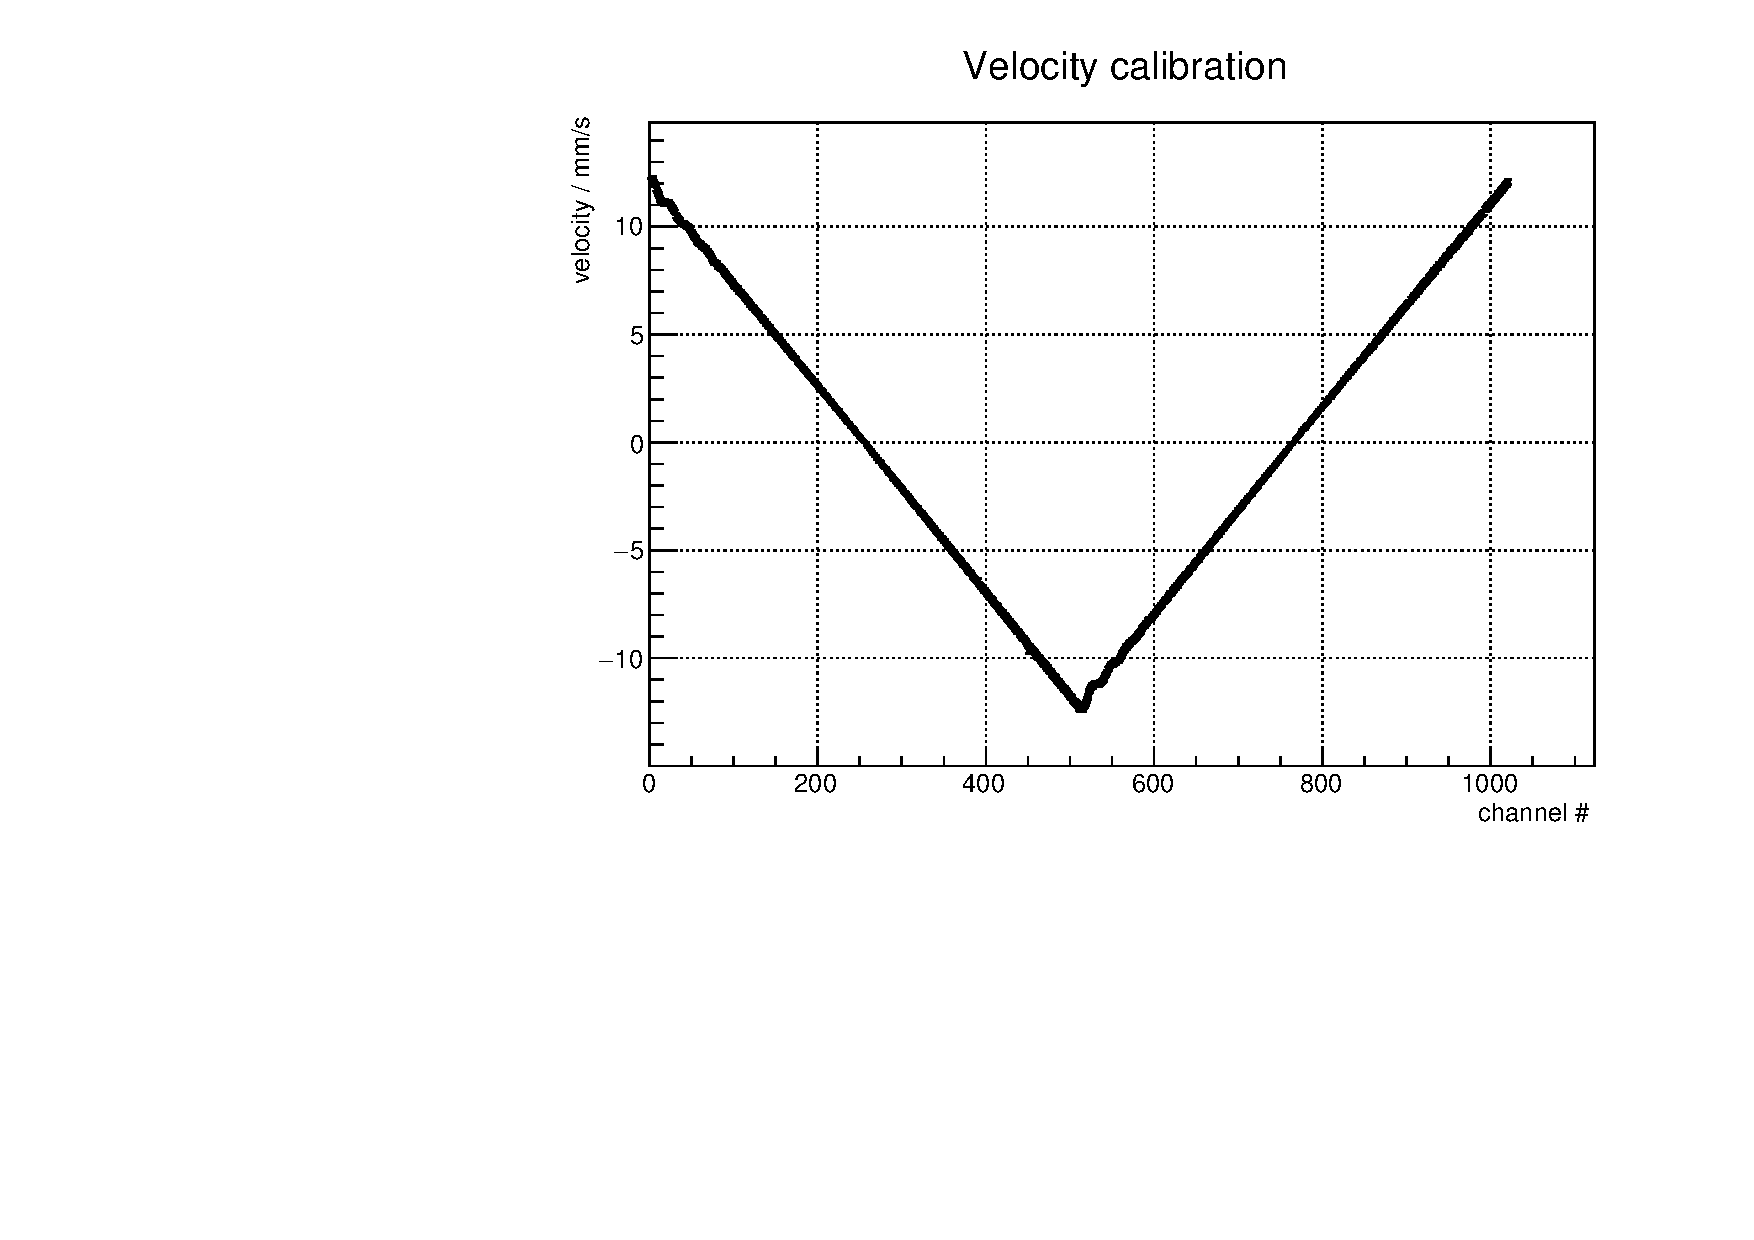
\includegraphics[scale = 0.5]{../plots/velocities.pdf}
\caption{Velocities}
\end{figure}


\FloatBarrier
\subsection{Spectra}
The following figures display the recorded spectra with gaussians fitted to the absorption peaks.

\begin{figure}
\label{fig:fe}
\centering
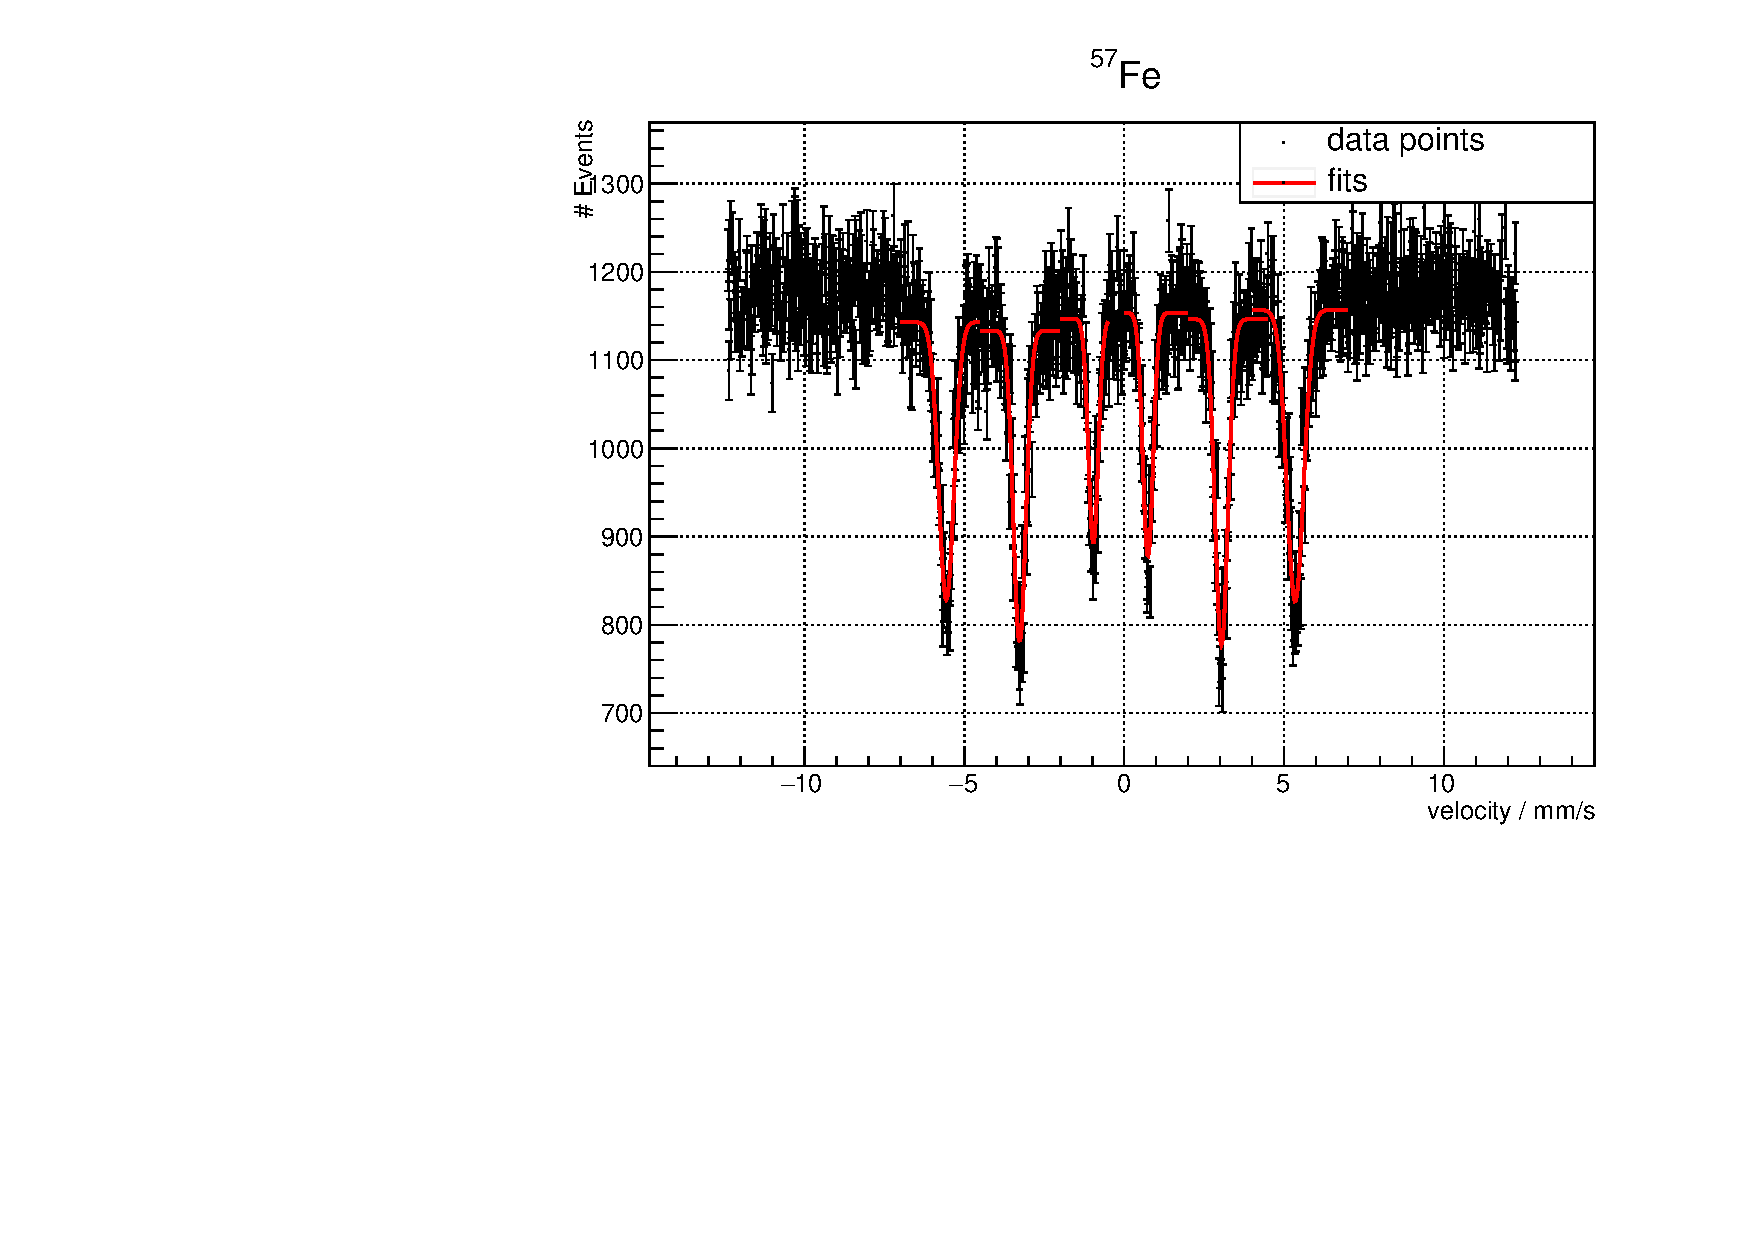
\includegraphics[scale = 0.5]{../plots/Fe57.pdf}
\caption{Velocities}
\end{figure}


\begin{figure}
\label{fig:vc}
\centering
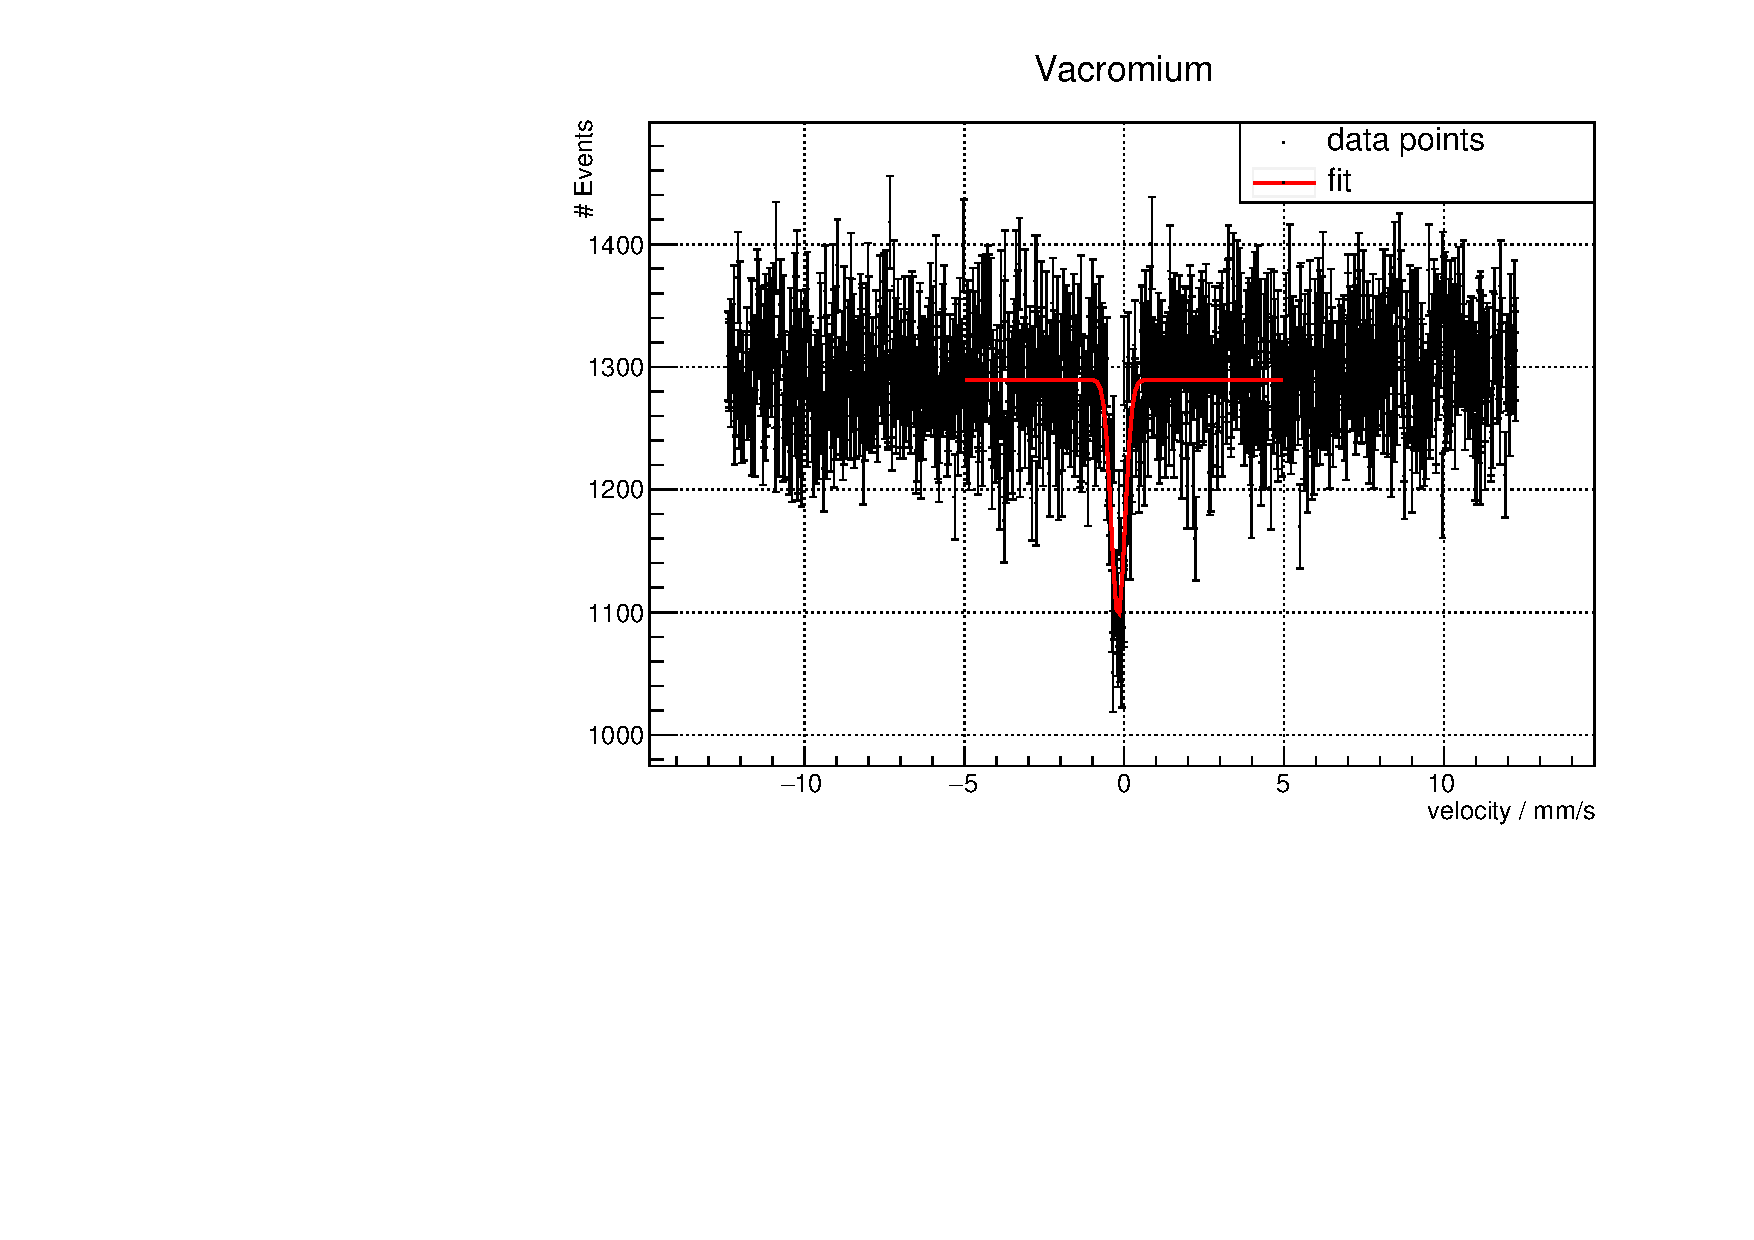
\includegraphics[scale = 0.5]{../plots/VC.pdf}
\caption{Velocities}
\end{figure}


\begin{figure}
\label{fig:fes}
\centering
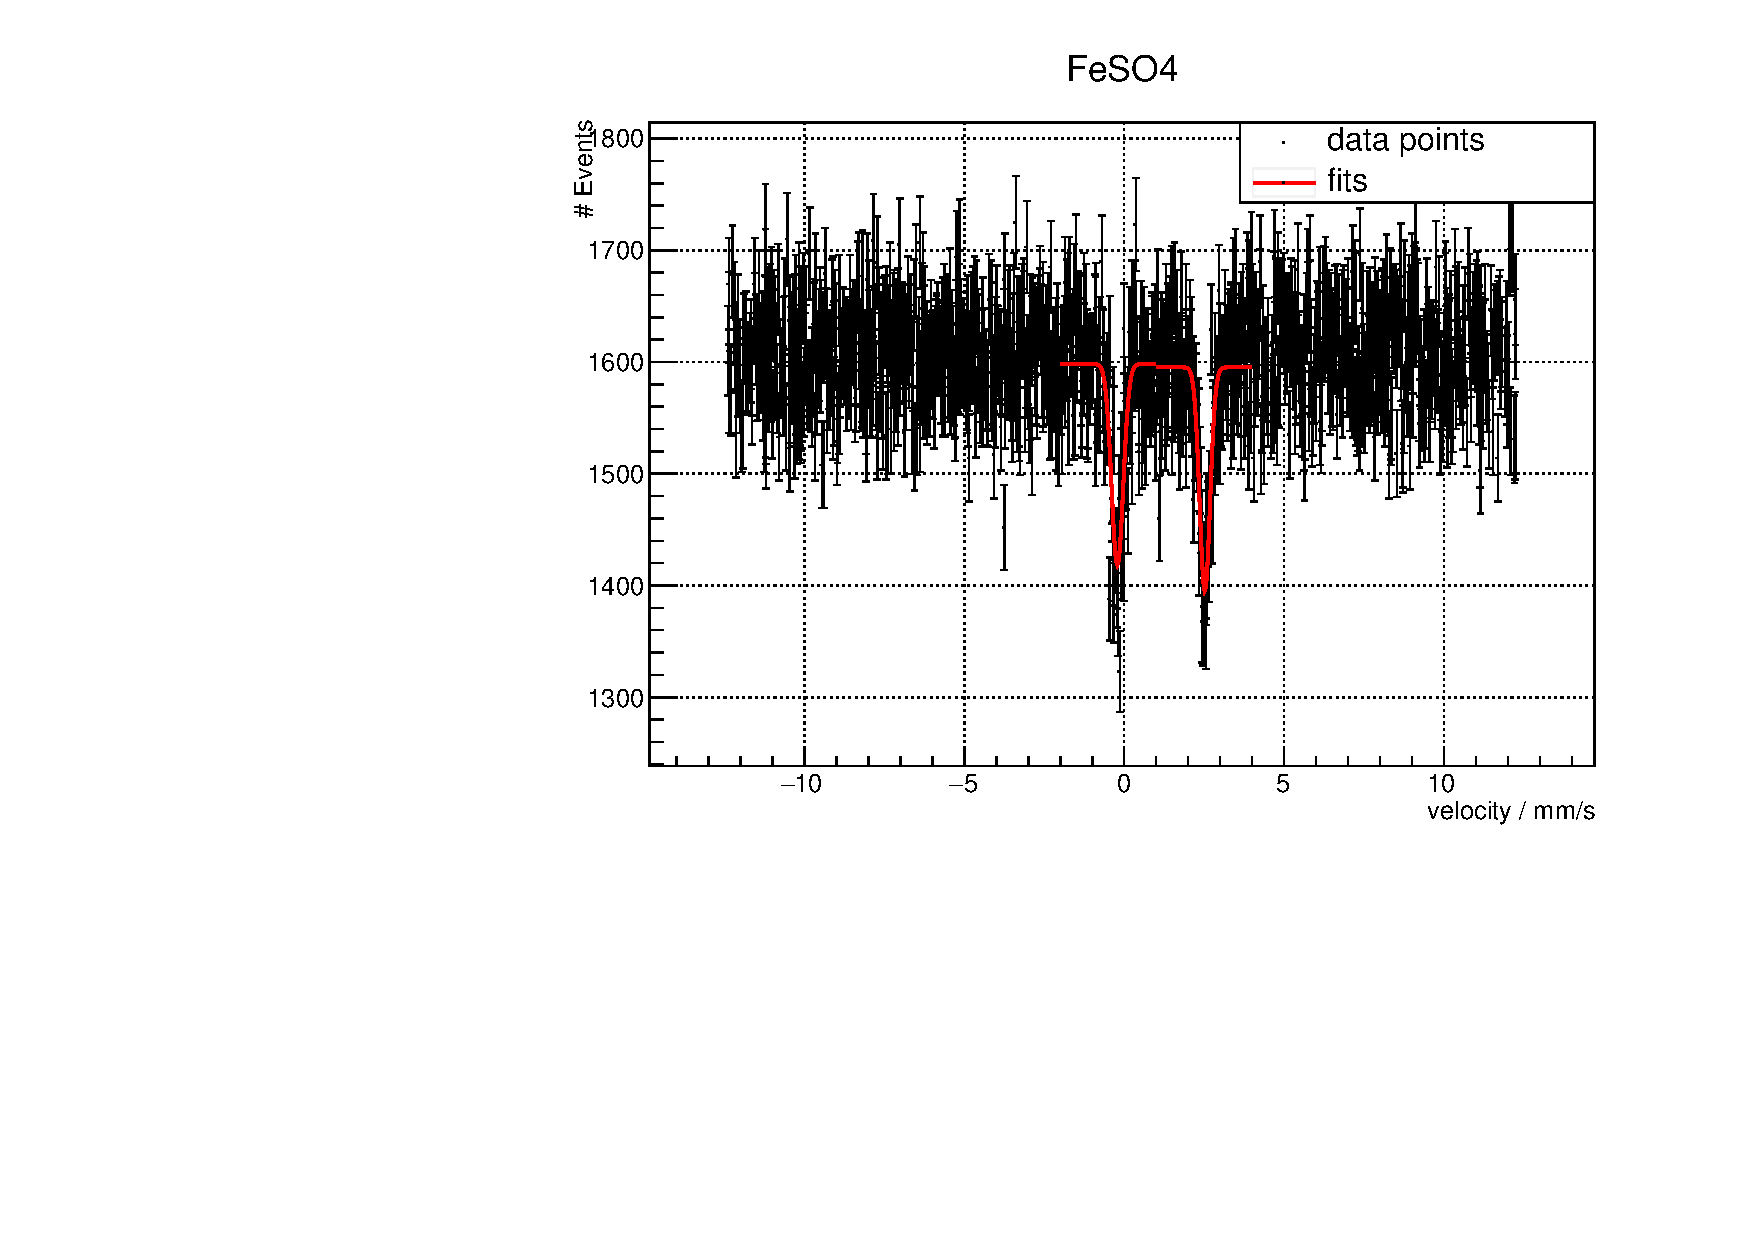
\includegraphics[scale = 0.5]{../plots/FeSO4.pdf}
\caption{Velocities}
\end{figure}


\begin{figure}
\label{fig:fep}
\centering
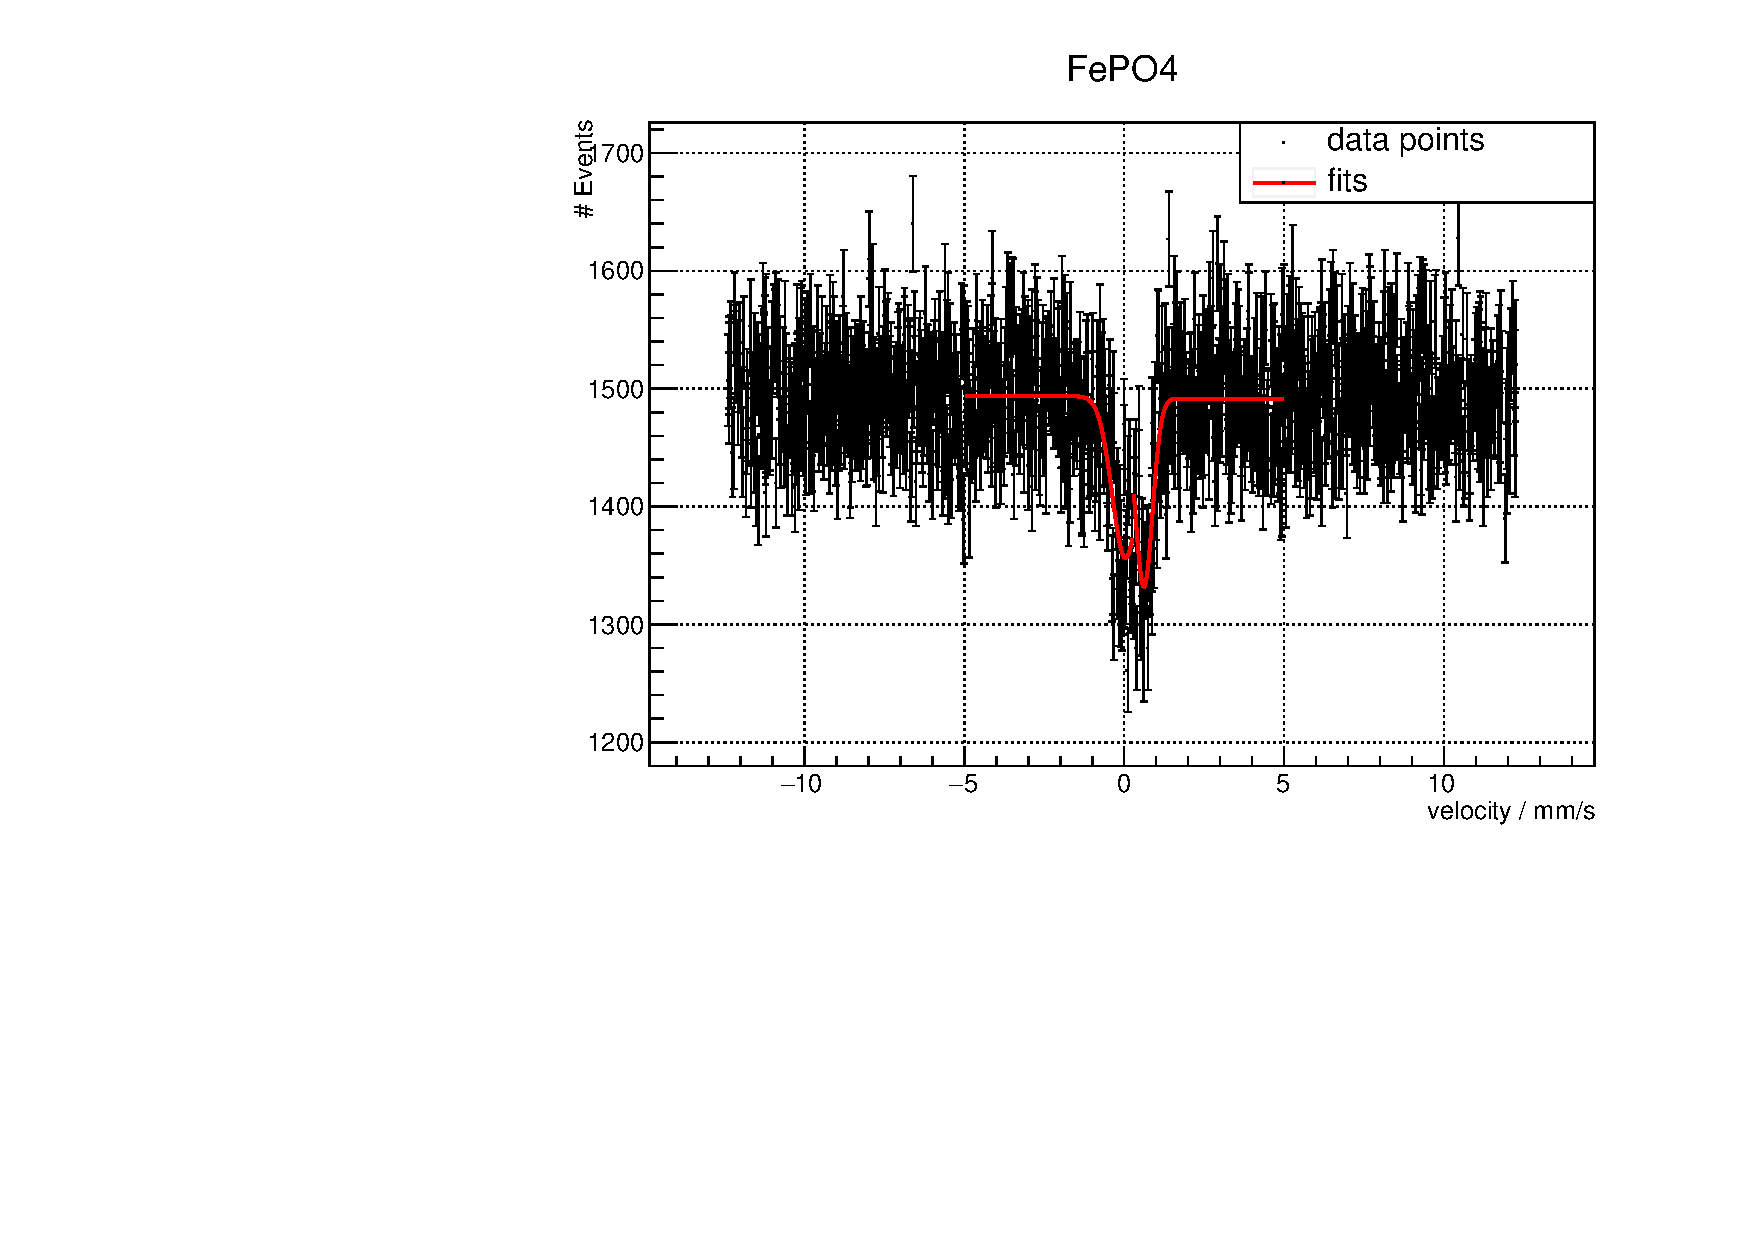
\includegraphics[scale = 0.5]{../plots/FePO4.pdf}
\caption{Velocities}
\end{figure}



\FloatBarrier

\subsection{Vacromium}

The chemical shift for the vacromium peak computes to:
$$\nu = -0.1907 \pm 0.0129 \ \text{mm}/\text{s}$$
The half width is:
$$v_{1/2} = 0.2529 \ \text{mm}/\text{s}$$
which corresponds to an energy of $\Delta E = 1.215 \cdot 10^{-8} \ \text{eV}$ for $14.4 \ \text{keV}$.\\
The lifetime of the excited state follows:

$$\tau = \hbar / \Gamma_0 = 2 \cdot \hbar / \Delta E = 108.4 \ \text{ns}$$


\subsection{Iron}
The fits give the following resonance velocities:

$$v_6-5.56 \pm  0.00789$$
$$v_5-3.27 \pm  0.00620$$
$$v_4-0.97 \pm  0.00800$$
$$v_3 0.74 \pm  0.00746$$
$$v_2 3.04 \pm  0.00607$$
$$v_1 5.34 \pm  0.00793$$

and thus
$$I = -0.11125 \ \text{mm}/\text{s}$$
for the chemical shift.

Since $v_1 = 2\cdot v_2 + v_3 = 0.006305 \text{mm}/\text{s}$ fulfills the criterium for the four possible parameter relations the best, it follows:

$$G = -v_2 - v_3 = -4.0066 \ \text{mm}/\text{s}$$
and
$$A = v_1 - v_2= 2.3044 \ \text{mm}/\text{s}$$

from these the internal magnetic field and moment follow:

$$B = \frac{G I_g E_0}{\mu_g c} = -33.8 \ \text{T}$$
$$\mu_e = \frac{A I_e E_0}{B c} = -4.912 \cdot 10^{-9} \text{eV}/\text{T}$$

There were no values provided in the literature for this lab, but this source\footnote{https://www.chemie.uni-hamburg.de/bibliothek/2003/DissertationPickardt.pdf} gives $-33 \ \text{T}$ and $-4.8768 \cdot 10^{-9} \text{eV}/\text{T}$, which is reasonably close to the values found here.

\subsection{Iron Compounds}
The field gradient of two different iron compounds is to be measured here.
\subsubsection{FeSO4}
The distance between the two peaks in the FeSO4 absorption spectrum is $\Delta v = 2.734 \ \text{mm}/\text{s}$ and thus the gradient is:
$$\frac{\partial^2 V}{\partial z^2} = 1.251 \cdot 10^{22} \ \text{V}/\text{m}/\text{m}$$

The chemical shift is $\nu = 1.954 \ \text{mm}/\text{s}$.


\subsubsection{FePO4}
For FePO4 the peaks are very close to each other. To resolve them, a single gaussian was fitted to both and the peak velocity of this fit used as the border between the fitting ranges of the single peaks.\\
With this the distance between peaks is $\Delta v = 0.5735 \ \text{mm}/\text{s}$ and the gradient:
$$\frac{\partial^2 V}{\partial z^2} = 1.251 \cdot 10^{22} \ \text{V}/\text{m}/\text{m}$$

The chemical shift is $\nu = 0.329 \ \text{mm}/\text{s}$.
